\begin{document}
%=================================================================
%                           Start Document
%=================================================================
\section{Implementation}
\lhead{Implementation} % section header
\setstretch{1.6}

\subsection{Software Refactoring}
As mentioned introduction wise this project builds upon the work and code base originally developed for FES with the LegoPress \cite{olivier_legopress_2014} and further developed by a previous student. However the code quality was poor with thousands of lines of code and multiple functionalities all implemented in one file and one class. Therefore before continuing on with the project a proper refactoring of the code was necessary.

The software is written in C++ in QT.

\subsubsection{Documentation}

In order to understand the code it was decided that the first step would be to create documentation, specifically graphical representations of the interactions and hierarchy. To accomplish the code was documented and edited so that it would be compatible with doxygen. Doxygen is a documentation generation tool that automatically creates software documentation from annotated source code in HTML.

\begin{figure} [H]
    \centering
    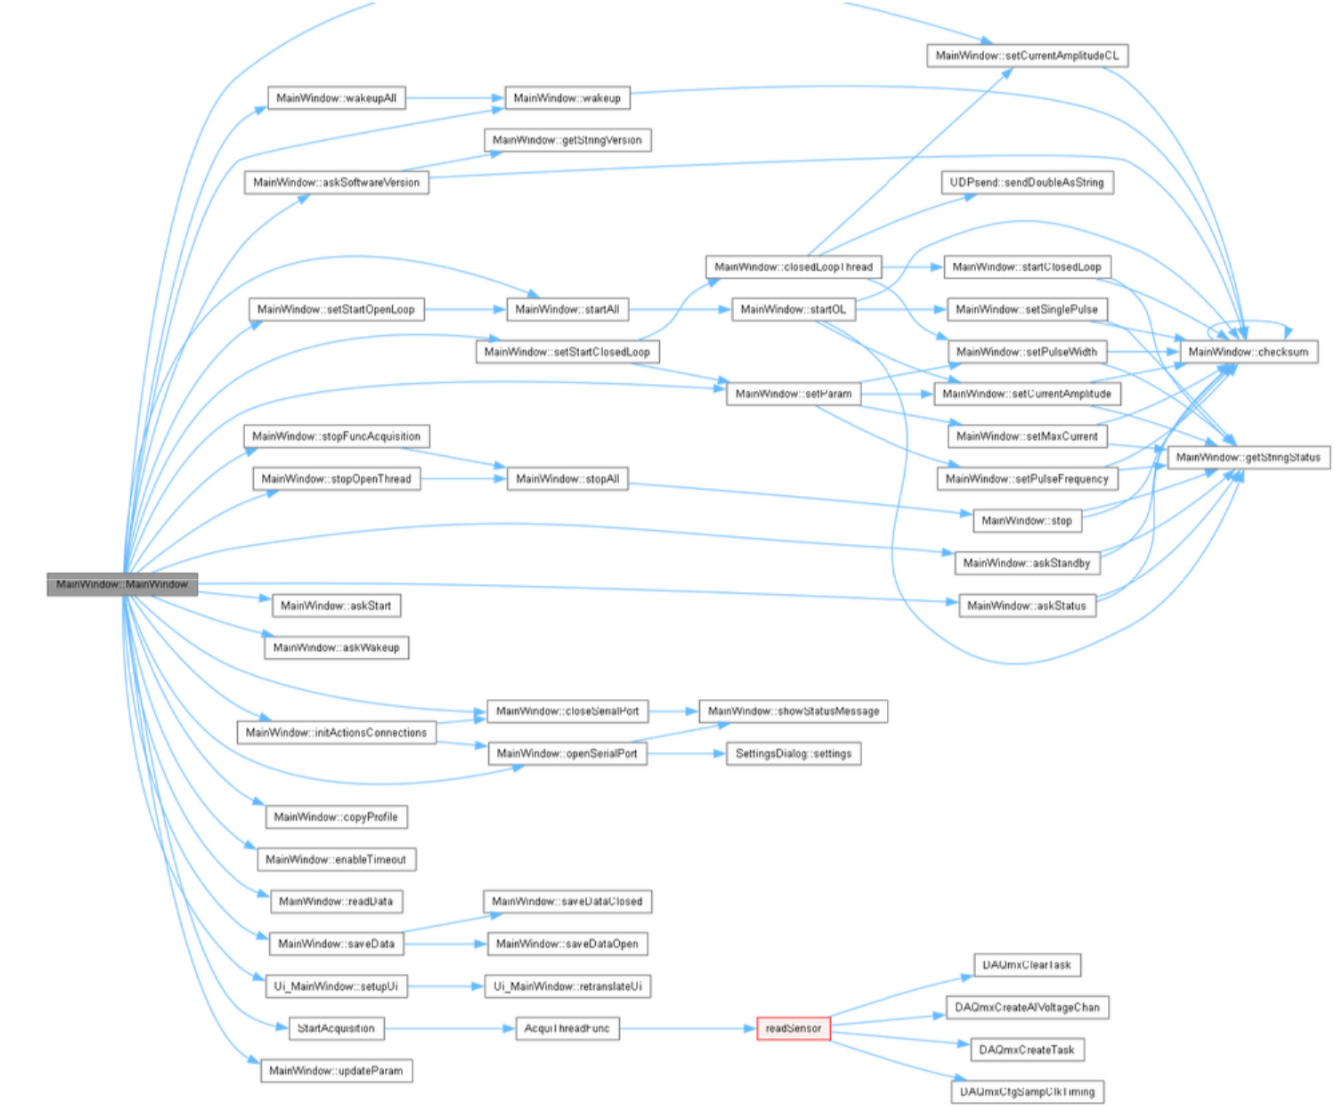
\includegraphics[width=0.9\linewidth]{images/oldDoxy.png}
    \caption{Original callgraph for mainwindow function before refactoring, generated by doxygen}
    \label{fig:oldDoxy}
\end{figure}

After the code had been documented and visualized in doxygen it became possible to see the call graphs and interactions such as in figure \ref{fig:oldDoxy}. This sped up the process of understanding the code thus laying important groundwork for the refactoring and modularization step.

\subsubsection{Modularization}
In order to improve the code quality a modularization of the code base was necessary. The code was refactored and split into classes largely based on the code quality principles laid out in Code Complete by Steve McConnel \cite{steve_mcconnell_code_nodate}. This includes having clearly defined, minimal interfaces. This is accomplished by using the signal slot mechanism inbuilt into QT, which allows for clear interfacing without circular interactions. Another core concept is organizing modules hierarchically, where higher-level modules depend on lower-level modules but not the revers. Where the top of the hierarchy is the class which manages the GUI named mainwindow.







As mentioned introduction wise this project builds on a code base developed at the REHassist lab. 

\subsection{Functional Electrical Stimulation Sequence}

\subsection{IMU Integration}

\subsection{Knee angle Extraction}

\subsection{Phase Detection}

\subsection{Closed loop}

\subsection{Functional Electrical Stimulation}

\subsubsection{Stimulation device: StimWave3}

\subsection{Closed Loop}

\subsubsection{Feedback: Inertial Measurement Unit}



gg
%=================================================================
%                           End Document
%=================================================================
\end{document}